\chapter{Qualitätssicherung}
\label{cha:qualitaetssicherung}
Um bei der Entwicklung von Applikationen eine hohe Qualität sicherstellen zu können und die Entwicklung zu beschleunigen,
müssen automatisierte Tests geschrieben werden (siehe mehr dazu unter \cite{online_quali_automatisiertetests}).

In diesem Kapitel wird erklärt, warum automatisierte Tests wichtig sind und wie in der Zukunft getestet werden muss, wenn
in einer Hybrid-Cloud-Umgebung gearbeitet werden soll.

Auch werden Tests für die jeweiligen Teilprogramme entwickelt und in den Buildprozess eingebunden.

\section{Allgemein}
Ein großer Vorteil der Cloud ist die schnelle und agile Entwicklung, die dort möglich ist. Problematisch ist es, wenn
zwar in schnelleren und kürzeren \textit{Sprints}, Versionen an den Geschäftspartner oder den Endkunden herausgegeben
werden können, diese aber gar nicht oder nur teilweise funktionieren.

Ein großes Ziel vieler Unternehmen ist die \glqq \textit{Time to Market}\grqq~zu reduzieren. Dennoch gilt die Regel,
dass nur Software, die vom Kunden genutzt werden kann, dem Unternehmen Geld bringt.

Eine Möglichkeit, diesem entgegen zu wirken und eine höhere Qualität der Software zu erreichen, ist der Aufbau von
automatisierten Tests. Frei nach dem Motto \glqq \textit{fail early and fail often}\grqq~wird die Software in nahezu
allen Funktionen vor dem eigentlichen Deployment getestet.

Der Testdurchlauf kann beliebig häufig neugestartet und wiederholt werden und das auch immer mit unterschiedlichen
Programmversionen.

Neben vielen weiteren haben automatisierte Tests den Vorteil, dass sie zu jeder Tages- und Nachtzeit durchlaufen
können und keine menschliche Person daneben sitzen muss, um den Test zu überprüfen. In der Regel wird die verantwortliche
Person nach einem Testdurchlauf über das Ergebnis benachrichtigt und kann dann eingreifen.

Allerdings sind automatisierte Tests nicht immer und für jede Anwendung geeignet. Michael Lüttel von der Deutschen
Flugsicherung sagte auf der iqnite-Konferenz in Düsseldorf \glqq Automatisierung macht nur dann Sinn, wenn sie mehr Aufwände
einspart als sie selbst erzeugt.\grqq\footnote{https://www.qz-online.de/news/uebersicht/nachrichten/vor-und-nachteile-von-automatisierten-software-tests-890130.html}.

\section{COBOL-Anwendung}
Für Unit Tests in COBOL hat, neben IBM, die Firma Compuware das Program
\path{Topaz for Total Test}\footnote{http://www.compuware.com/en\_us/products/topaz-for-total-test.html} entwickelt.
Dabei handelt es sich um ein Testprogramm, um Testfälle zu definieren und diese bei Quellcodeänderungen automatisch
auszuführen.

Da die vorliegende COBOL-Anwendung nicht komplett selbstgeschrieben wurde und nur die Schnittstellen mittels IBM Application
Discovery definiert wurden, werden keine Tests geschrieben.

Es wird lediglich die definierte Schnittstelle getestet indem die richtigen Parameter an die Anwendung geschickt werden
um anschließend zu überprüfen, ob die Daten richtig in die Datenbank geschrieben, abgeändert oder gelesen wurden.

Diese Tests werden am Anfang durchgeführt, und da sich die COBOL-Anwendung weder ändert noch angepasst wird, müssen sie
nicht wiederholt werden. Eine Einbindung in einen Buildprozess ist deshalb nicht nötig.

\section{Frontend}
Da es sich beim Frontend um eine Applikation auf Basis von HTML, CSS und JavaScript handelt und diese im Browser angezeigt
werden, werden für das Frontend Headless-Browser-Tests erstellt.

Bei Headless-Browser-Tests handelt es sich um Tests, welche die Webseite mit Hilfe einem vorgegebenem Pfad virtuell
durchklicken und das resultierende DOM-Objekt mit der Vorgabe vergleichen.

Bei der Überprüfung des DOM-Objektes kann lediglich ein kleiner Teil vorgegeben werden, welcher überprüft werden soll. So
ist es zum Beispiel möglich zu testen, ob die Überschrift, gängigerweise in einem \path{<h1>}-Tag, mit der gewünschten
übereinstimmt.

Die Tests für das Web-Frontend werden mit CasperJS\footnote{http://casperjs.org} erstellt und mit dem Testrunner
Karma\footnote{https://karma-runner.github.io/1.0/index.html} ausgeführt.

Ein einfacher Test einer Webseite zur Überprüfung der angegebenen Überschrift ist in Listing
\ref{Einfacher Test in CasperJS} auf Seite \pageref{Einfacher Test in CasperJS} zu sehen.

\begin{lstlisting}[language=JavaScript, caption=Einfacher Test in CasperJS, label=Einfacher Test in CasperJS]
var casper = require('casper').create();

casper.start('http://domain.tld/page.html', function() {
    if (this.exists('h1')) {
        this.echo('the heading exists');
    }
});

casper.run();
\end{lstlisting}

Da das Web-Frontend lediglich eine Seite besitzt, wird kein Wechsel der URL benötigt. So kann mittels CasperJS die
Startseite aufgerufen werden und anschließend die Überschriften der vier Boxen überprüft werden und ob die Einträge
der einzelnen Attribute mit \textit{no data available} beschriftet sind.

Außerdem wird getestet, ob das Betätigen des Buttons \path{START POLLING} nach maximal 15 Sekunden Werte für die Attribute
anzeigt. Falls dies zutrifft wird ein Screenshot erstellt und in der Testumgebung abgelegt. Dies dient der späteren manuellen
Überprüfung.

Mit diesem Test wird indirekt auch der Secure Gateway, der Java-Wrapper, die COBOL-Anwendung und die Verbindung zur
Datenbank getestet.

Der Testrunner \path{Karma} ist deshalb interessant, da mit CapserJS lediglich einzelne Testcases geschrieben werden
können. Mit einem Testrunner können die einzelnen Testcases, welche immer nur einen Teil der Anwendung betesten,
zusammengeführt und nacheinander ausgeführt werden. Alternativ müsste jeder Testcase einzelnd ausgeführt werden.

Das Ausführen der Tests wird in der Toolchain hinterlegt und ist somit ein Teil des Deploymentvorgangs innerhalb von
Bluemix.

Alle Tests können im GitHub-Repository des Web-Frontends eingesehen werden.

\section{Backend}
Das Backend (der Java-Wrapper) wurde in der Programmiersprache Java entwickelt. Die Tests werden deshalb in
JUnit\footnote{http://junit.org} erstellt.

Bei den Tests für das Backend handelt es sich um automatisierte Testaufrufe des REST-Interfaces mit Überprüfung der
gelieferten Rückgabewerte.

Um JUnit-Tests schreiben zu können wird dem Projekt die JUnit-Library hinzugefügt. Im Anschluss wird ein Unterordner mit
Namen \path{/tests} im Projekt angelegt. Dort werden alle Testklassen gespeichert.

In Listing \ref{Einfacher JUnit Test} auf Seite \pageref{Einfacher JUnit Test} ist ein einfacher JUnit-Test zu sehen,
welcher die Methode \path{multiply} testet, welche zwei Parameter übergeben bekommt. Beide Parameter werden anschließend
multipliziert und das Ergebnis zurück gegeben. In diesem Beispiel wird getestet, ob eine Zahl multipliziert mit \textit{0}
auch immer \textit{0} ergibt. Ob die entwickelte Funktion also korrekt rechnet.

\begin{lstlisting}[language=java, caption=Einfacher JUnit Test, label=Einfacher JUnit Test]
public class OwnTests {

    @Test
    public void multiplicationOfZero() {
        OwnClass tester = new OwnClass(); // OwnClass is tested

        // assert statements
        assertEquals("10 x 0 must be 0", 0, tester.multiply(10, 0));
        assertEquals("0 x 10 must be 0", 0, tester.multiply(0, 10));
        assertEquals("0 x 0 must be 0", 0, tester.multiply(0, 0));
    }
}
\end{lstlisting}

Im geschrieben Backend werden die einzelnen REST-Endpunkte mit den richtigen und auch falschen Parametern aufgerufen
und der Rückgabewert mit dem Erhofften verglichen.

Die Tests des Backends können in der Hybrid-Cloud-Architektur auf zwei Arten automatisch durchgeführt werden.

\begin{itemize}
    \item Während dem Build in der Toolchain (Bluemix)
    \item Nach dem Build mittels RTC direkt auf dem Mainframe
\end{itemize}

Im Folgenden wird kurz erklärt, wie die geschriebenen Tests in die beiden Programme eingebunden werden können.

\subsection{Mittels Toolchain testen}
Für das automatische Ausführen der Tests in der Toolchain in Bluemix wird die in Kapitel \ref{subsec:einrichten_der_toolchain}
auf Seite \pageref{subsec:einrichten_der_toolchain} angelegte Toolchain um einen Block für automatisierte Tests erweitert.

Dafür wird eine neue Phase hinzugefügt. Als Name wird hier \path{Test Stage} gewählt. Der Eingabetyp ist
\path{Buildartefakt}. Dies wird benötigt, damit auch das kompilierte Artefakt getestet werden kann.

In der Kategorie \path{JOBS} wird ein neuer hinzugefügt. Der Jobtyp ist \path{Test}. Es erscheint ein neuer Bereich mit
weiteren Konfigurationsmöglichkeiten.

Als Testtyp wird hier \path{Einfach} ausgewählt und als Befehl zum Starten des JUnit Tests der \path{java}-Befehl
eingetragen.

\begin{lstlisting}[language=bash, caption=Ausführen von JUnit Tests, label=Ausführen von JUnit Tests]
    java -cp .:/usr/share/java/junit.jar org.junit.runner.JUnitCore
\end{lstlisting}

Nach der Speicherung der Stage wird diese in der Toolchain ans Ende hinzugefügt. Nun muss sie noch zwischen die
\textit{DEPLOY}- und \textit{BUILD}-Stage geschoben werden. Siehe dazu Abbildung \ref{fig:toolchain_teststage} auf Seite
\pageref{fig:toolchain_teststage}.

\begin{figure}[h]
  \centering
    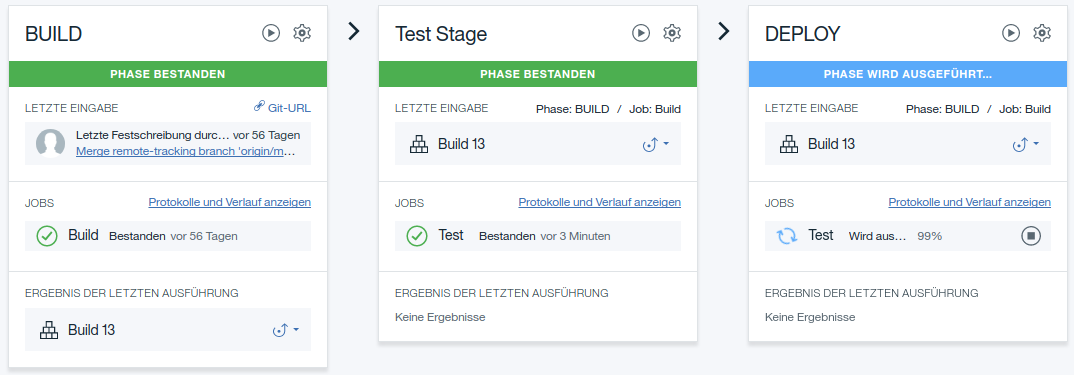
\includegraphics[scale=0.35]{images/kapitel_5/toolchain_teststage.png}
  \caption{Übersicht der Toolchain mit Test Stage}
  \label{fig:toolchain_teststage}
\end{figure}

Nach der Einrichtung wird die Test Stage nach jedem \path{push} in das zugehörige Git-Repository automatisch ausgeführt.
Im Anschluss wird die Anwendung (wie in der Abbildung zu sehen), automatisch auf das System installiert. Der komplette
Durchlauf der Toolchain sollte je nach Anzahl von Tests und Anzahl von Klassen in der Java-Anwendung wenige Minuten dauern.

Wichtig ist dabei die Reihenfolge. Im Gegensatz zum Test mit RTC (im folgenden Kapitel), wird das Backend immer getestet,
bevor es auf dem System installiert wird. Wenn ein oder mehrere Tests schiefgehen, wird auch die neue Version nicht
installiert. Dies bedeutet auch keinen Ausfall der Anwendung, wenn etwas falsch programmiert wurde.

\subsection{Mittels UCD testen}
Das Testen der Java-Anwendung mittels UCD wird in der Weboberfläche von UCD eingerichtet. Dabei wird ein neuer Task
hinzugefügt, welcher die Anwendung selbstständig testen kann.

Da der Test nicht in den Deploymentvorgang eingebaut wird, muss der Task bei Bedarf manuell gestartet werden. Es ist
sinnvoll dies immer nach einem Deployment zu tun, damit sichergestellt werden kann, dass die Anwendung korrekt funktioniert.

In Abbildung \ref{fig:ucd_teststage} auf Seite \pageref{fig:ucd_teststage} ist der eingerichtete Task mit Namen
\textit{Insurance-Backend-Interface-Integration.Test} zu sehen.

\begin{figure}[h]
  \centering
    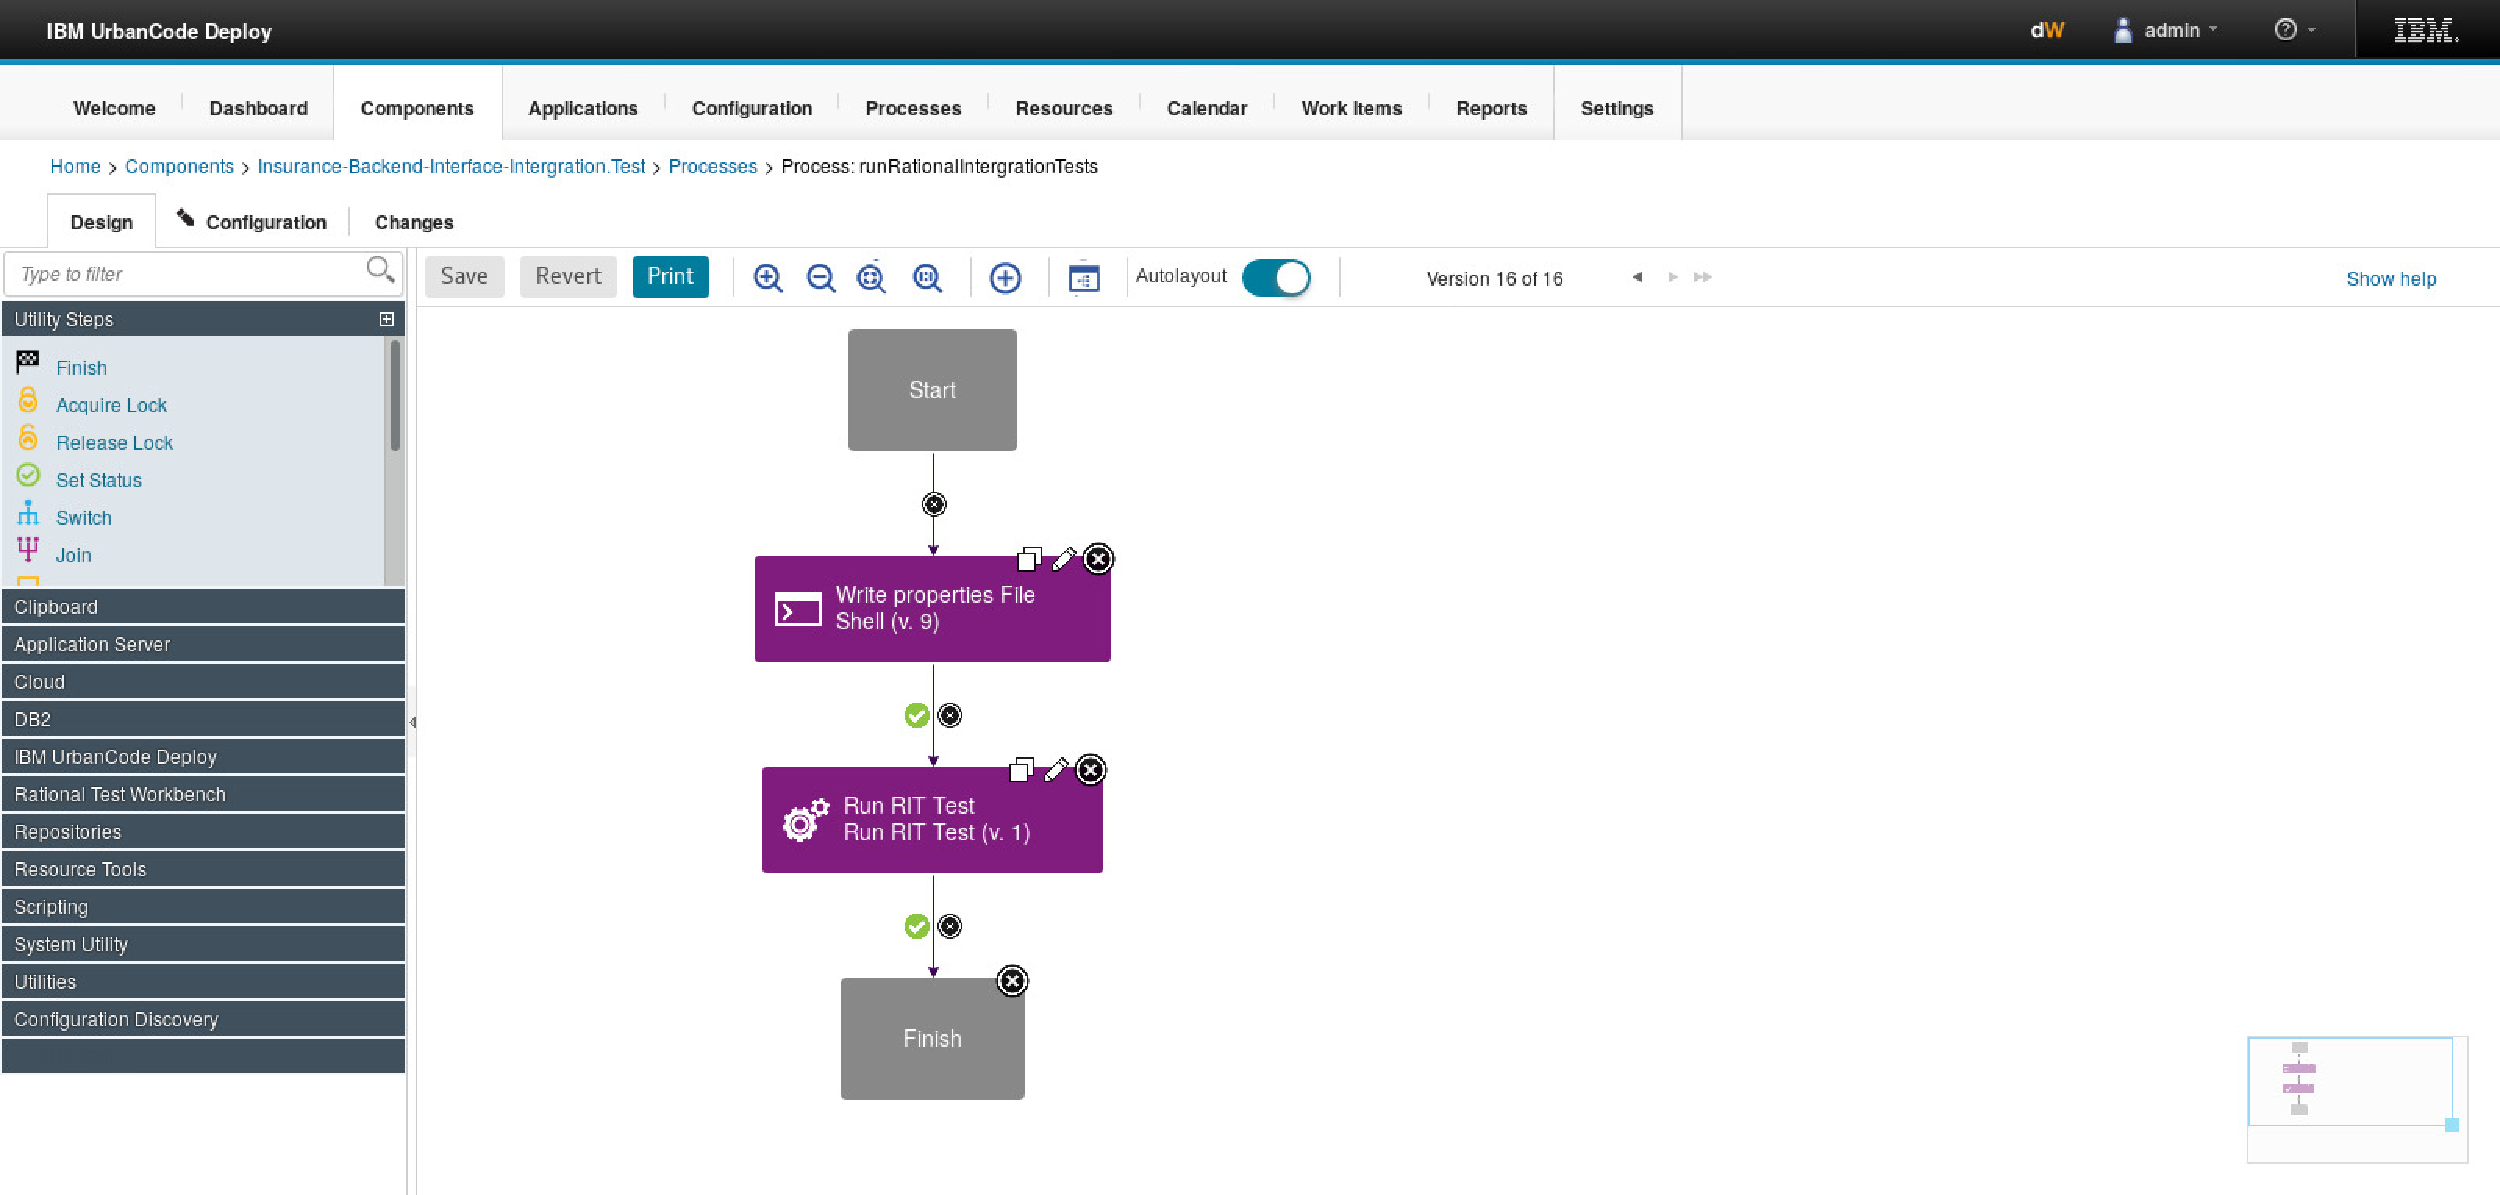
\includegraphics[scale=0.3]{images/kapitel_5/ucd_teststage.pdf}
  \caption{Übersicht des Test-Tasks in UCD}
  \label{fig:ucd_teststage}
\end{figure}

In diesem Task wird zuerst eine Konfigurations-Datei angelegt, welche vom Testscript ausgelesen wird. Bei der Konfiguration
handelt es sich um Parameter wie Speicherort der Anwendung oder verwendete CICS-Region. Dies ist wichtig, damit das
Testscript die richtige Anwendung testen kann.

Das Testscript startet ein Programm mit dem es möglich ist REST-Interfaces zu testen. Dazu wird das installierte
Java-Interface mit vordefinierten Parametern aufgerufen und die Antwort mit den geforderten verglichen. Wenn alle Aufrufe
korrekt sind, wird der Administrator benachrichtigt.

Sollte ein Test allerdings fehlschlagen wird automatisch ein \textit{rollback} eingeleitet, welcher die letzte funktionierende
Anwendung installiert. Zusätzlich wird der Administrator benachrichtigt. Dieses Vorgehen hat den Vorteil, dass eine
Anwendung die nicht richtig funktioniert bis maximal nach dem Testdurchlauf auf dem System installiert ist und keinen
größeren Schaden anrichten kann.

Nach jedem Start des Tests in UCD wird ein \textit{Execution}-Log angelegt. Dieser ist in Abbildung
\ref{fig:ucd_teststage_duration} auf Seite \pageref{fig:ucd_teststage_duration} zu sehen.

\begin{figure}[h]
  \centering
    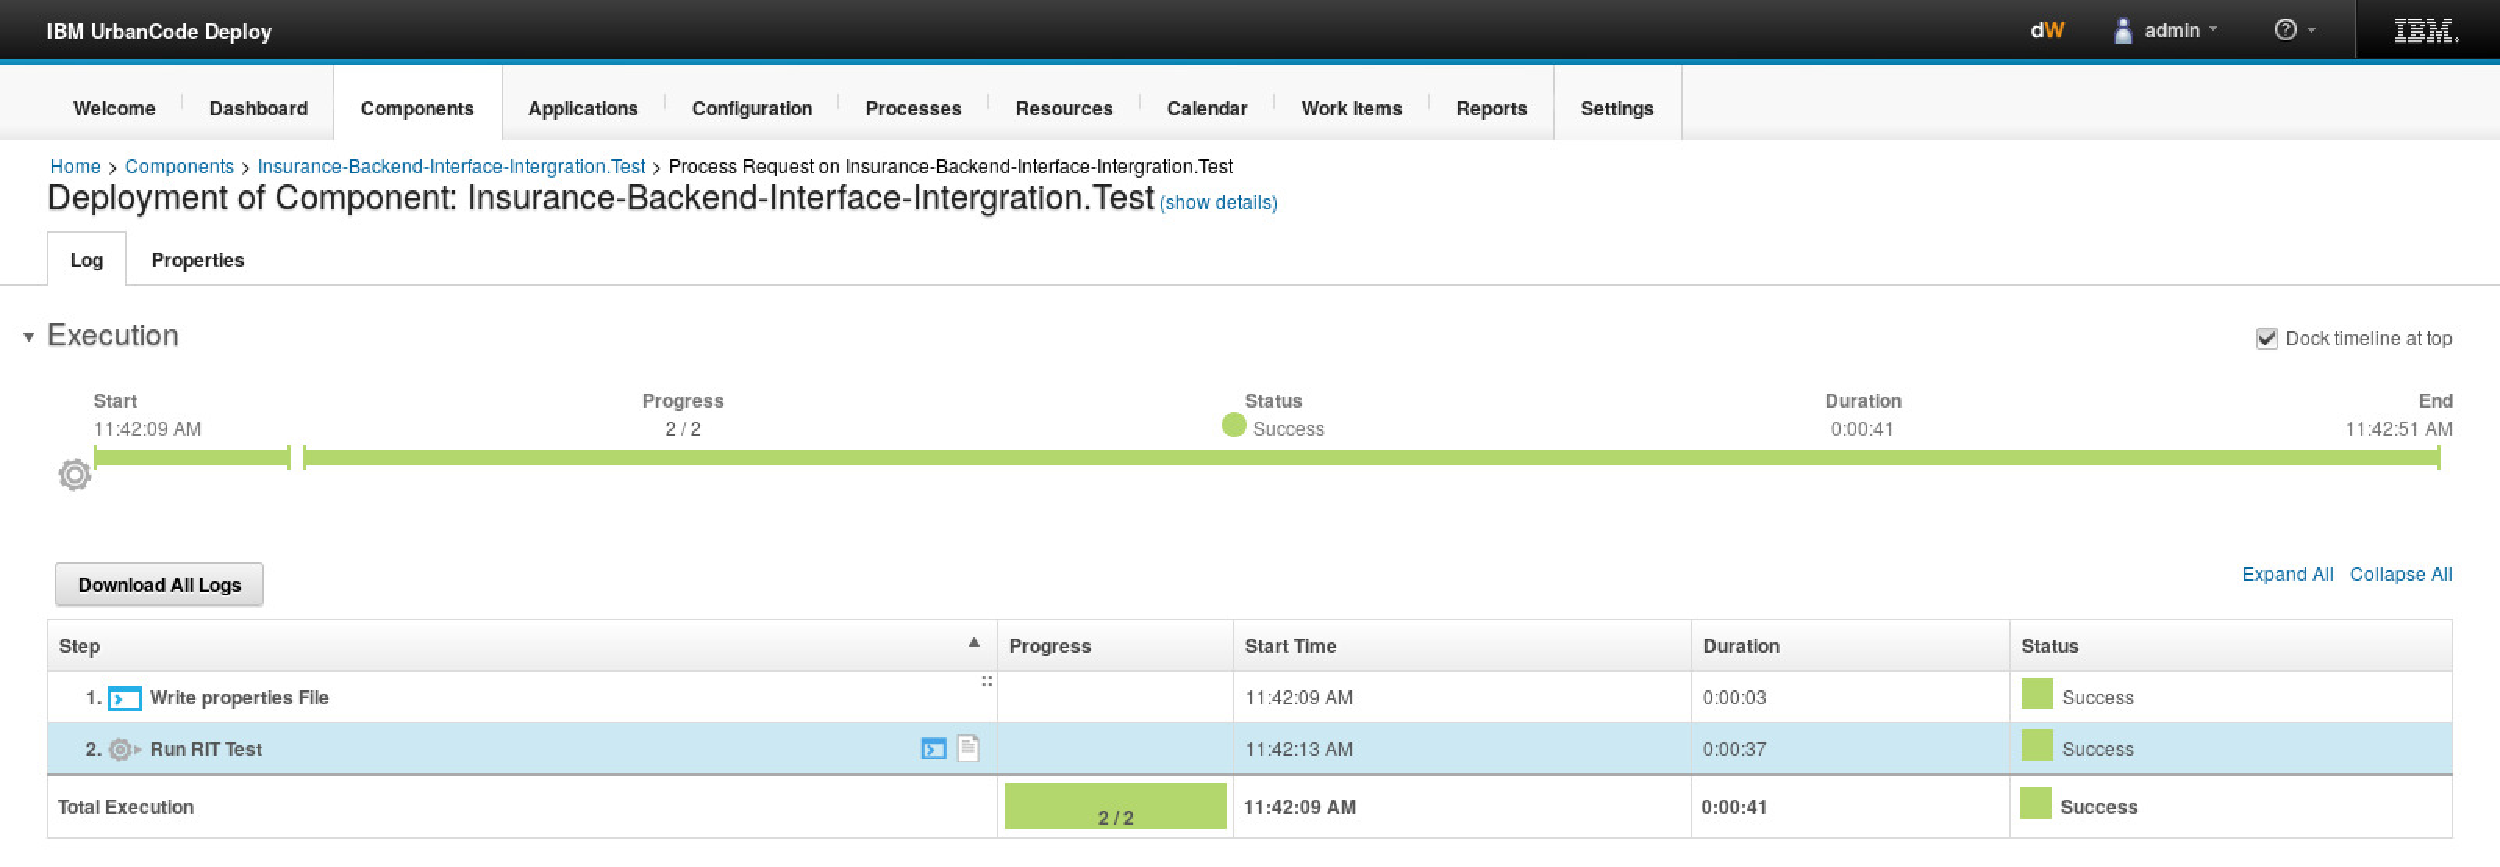
\includegraphics[scale=0.3]{images/kapitel_5/ucd_teststage_duration.pdf}
  \caption{Übersicht eines Testdurchlaufs in UCD}
  \label{fig:ucd_teststage_duration}
\end{figure}

In diesem Log kann eingesehen werden, wann der Test gestartet wurde, wie lange ein Step gebraucht hat und wie lange der
Test insgesamt gelaufen ist. In diesem Beispiel hat das Anlegen der Konfigurations-Datei nur drei Sekunden gedauert und
der komplette Test lediglich 37 Sekunden.

Insgesamt hat der Testdurchlauf im Beispiel nur 41 Sekunden gedauert und beide Steps wurden erfolgreich durchlaufen. In
einem Fehlerfall wäre im Log ersichtlich welcher Step fehlgeschlagen ist und warum.

\section{Smartphone App}
Da es sich bei den beiden Smartphone-Apps um WebView-Applikationen handelt und diese beim Start das schon betestete Web-Frontend
laden und anzeigen, decken die Frontend-Tests schon den größten Teil ab. Auch die Logik ist schon betestet.

Bei der Android- sowie bei der iOS-App gibt es allerdings wenige Zeilen Code in nativer Programmiersprache. Die
Funktion dieser muss allerdings getestet werden.

Die Tests der beiden Anwendungen werden in keinen Buildprozess eingebunden, da die Anwendungen seperat auf dem jeweiligen
Store hochgeladen oder bei Bedarf über andere Kanäle verteilt werden.

In den folgenden beiden Kapiteln wird der Aufbau der Tests genauer erklärt.

\subsection{Android-App}
Da die Android-App, genau wie das Backend, in Java geschrieben ist, werden auch hierfür die Tests in JUnit geschrieben.

Dafür wird in dem Android Studio Projekt im Verzeichnis \path{/app} in der Datei \path{build.gradle} im Bereich
\path{dependencies} die Dependency von JUnit hinzugefügt. Anschließend wird das Projekt neu gebaut, um die neue Dependency
automatisch herunter zu laden.

\begin{lstlisting}[language=bash, caption=Dependency hinzufügen, label=Dependency hinzufügen]
    androidTestCompile 'junit:junit:+'
\end{lstlisting}

Im Anschluss wird im Ordner \path{/app/src/} ein Ordner namens \path{test} hinzugefügt. In diesem werden alle Testcases
abgelegt, die ausgeführt werden sollen. Ein einfacher Test in Android sieht ähnlich einem Test in \path{Plain Java} aus.

\begin{lstlisting}[language=java, caption=Einfacher Test für Android, label=Einfacher Test für Android]
    public class ExampleUnitTest {
        @Test
        public void addition_isCorrect() throws Exception {
            assertEquals(4, 2 + 2);
        }
    }
\end{lstlisting}

Dieser statische Test prüft, ob die mathematische Gleichung \begin{math} 2+2 = 4 \end{math} zu jeder Zeit erfüllt ist.

Für die Android-Applikation ist es sinnvoll zu prüfen, ob auch die richtige URL geladen wird. Also ob das WebView-Layout
die richtige Webseite geladen hat und diese auch angezeigt wird.

Auch ist es sinnvoll während dem Test automatisiert ein Screenshot zu erstellen, welcher das Web-Frontend zeigt. So können
ggf. Fehler in der Größenanpassung behoben werden.

\subsection{iOS-App}
Für die iOS-App, welche in Swift 3 enwtickelt ist, werden die Tests in iOS Unit Testing geschrieben.

Dafür wird ein \path{Test Target} angelegt. Dies geschieht über das Hinzufügen einer \path{Unit Test Class} direkt in
XCode. Siehe dafür Abbildung \ref{fig:xcode_createtest} auf Seite \pageref{fig:xcode_createtest}.

\begin{figure}[h]
  \centering
    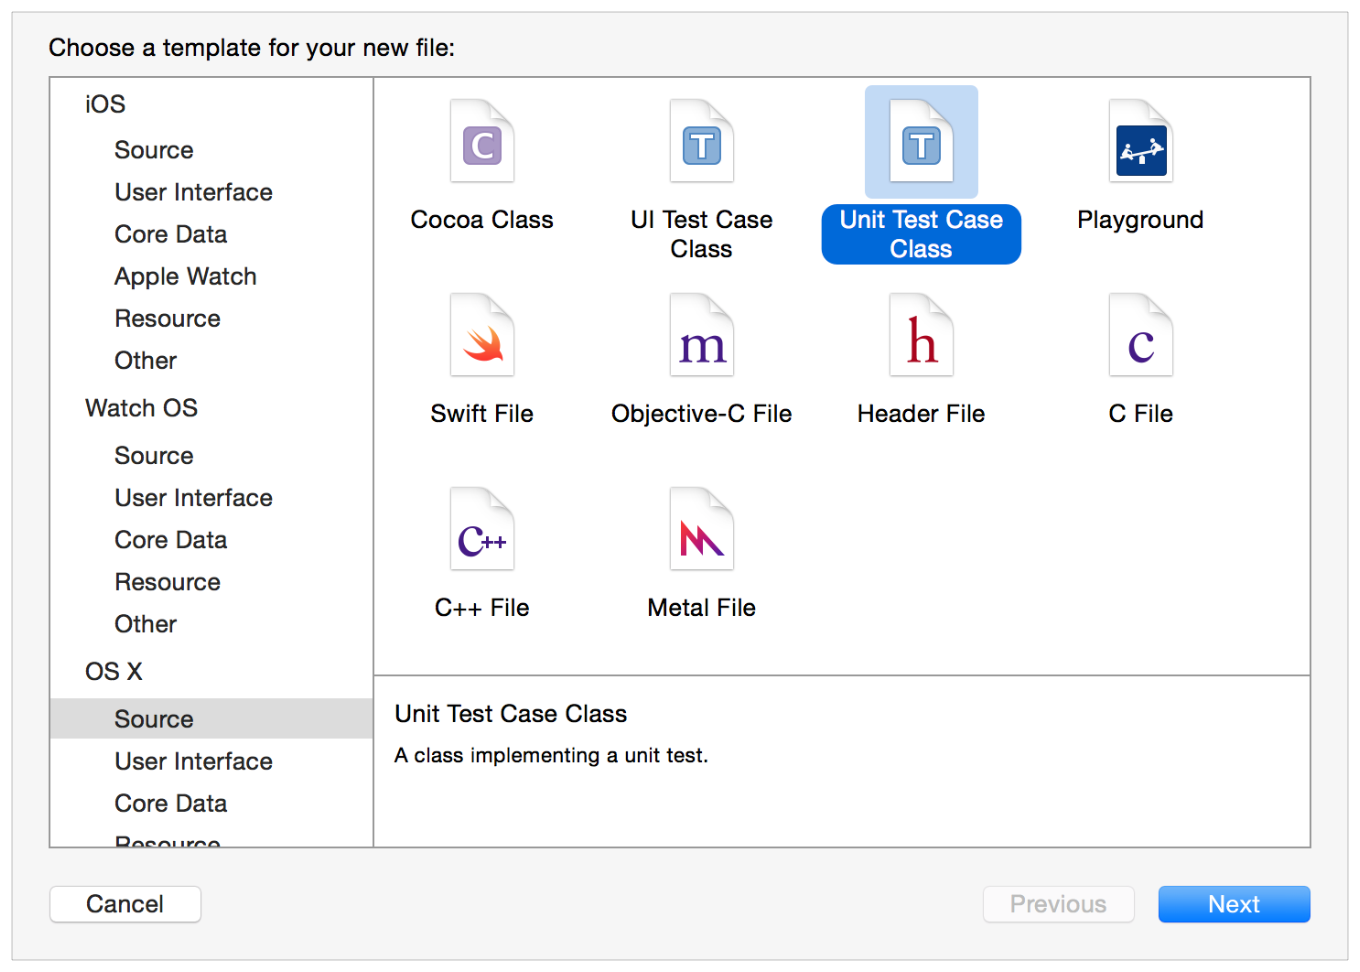
\includegraphics[scale=0.5]{images/kapitel_5/xcode_createtest.png}
  \caption{Hinzufügen einer Test Klasse in XCode}
  \label{fig:xcode_createtest}
\end{figure}

Ein beispielhafter Test kann in Listing \ref{Einfacher Test für iOS} auf Seite \pageref{Einfacher Test für iOS} eingesehen werden.

\begin{lstlisting}[language=c, caption=Einfacher Test für iOS, label=Einfacher Test für iOS]
    func testScoreIsComputed() {
      let guess = 5
      let value = 5

      XCTAssertEqual(guess, value, "Score guessed wrong")
    }
\end{lstlisting}

Dieser beispielhafte Test prüft, ob der Wert welcher geschätzt wurde (\path{guess}) gleich dem Wert ist, der fest gesetzt
wurde (\path{value}). Falls nicht, wird die definierte Fehlermeldung ausgegeben.

Wie auch in der Android-App wird hier lediglich getestet, ob das WebView-Layout die richtige Webseite lädt und auch
anzeigt. Der Rest wurde durch die Tests im Web-Frontend abgedeckt.